\documentclass{beamer}

\usepackage{soul}
\usepackage{graphicx}
\usepackage{tikz-cd}
\usepackage{tikz}
\usepackage{amssymb}
\usepackage{wasysym}
\usepackage{booktabs}
\usepackage{cases}
\usepackage{indentfirst}
\usepackage{graphicx}
\usepackage{adjustbox}
\newcommand{\new}[1]{\color{blue}#1\normalcolor}
\newcommand{\delete}[1]{}
\newcommand{\change}[1]{\color{black}#1\normalcolor}
\newcommand{\rev}[1]{\color{black}#1\normalcolor}
\graphicspath{{PresentationFigsMovies/},{Cassandra/Fig1},{Cassandra/Fig2},{Cassandra/Fig3},{Cassandra/Fig4},{Cassandra/Fig5},{Cassandra/Fig6}}


% VECTOR AND MATRIX NOTATION
\newcommand{\V}[1]{\boldsymbol{#1}}                 % vector notation
\newcommand{\M}[1]{\boldsymbol{#1}}
\newcommand{\Lop}[1]{\boldsymbol {\mathcal{#1}}}
\def\checkmark{\tikz\fill[scale=0.4](0,.35) -- (.25,0) -- (1,.7) -- (.25,.15) -- cycle;}
\def\xmark{\tikz[scale=0.23] {
    \draw[line width=0.7,line cap=round] (0,0) to [bend left=6] (1,1);
    \draw[line width=0.7,line cap=round] (0.2,0.95) to [bend right=3] (0.8,0.05);}}
\global\long\def\Ac{A_\text{cyto}}
\global\long\def\Pc{P_\text{cyto}}
\newcommand{\CDC}[1]{#1_{\text{c}}}
\newcommand{\6}[1]{#1_{\text{6}}}
\newcommand{\3}[1]{#1_{\text{3}}}
\newcommand{\CHIN}[1]{#1_{\text{ch}}}
\global\long\def\kon{k^\text{on}}
\global\long\def\koff{k^\text{off}}
\global\long\def\kf{k^+}
\newcommand{\Tot}[1]{#1^\text{(Tot)}}
\global\long\def\Dt{\partial_t}
\global\long\def\Dthat{\partial_{\hat{t}}}
\global\long\def\Dx{\partial_x}
\global\long\def\Dxhat{\partial_{\hat{x}}}
\global\long\def\MChinC{P_\text{cyto}}
\global\long\def\MChin{P_1}
\global\long\def\PChin{P_n}
\global\long\def\MAC{A_\text{cyto}}
\global\long\def\MA{A_1}
\global\long\def\PA{A_n}
\global\long\def\CDCy{C_\text{cyto}}
\global\long\def\CD{C}
\global\long\def\kp{k^\text{p}}
\global\long\def\kdp{k^\text{dp}}
\global\long\def\kI{k^\text{I}}
\global\long\def\kE{k^\text{E}}
\newcommand{\A}[1]{#1_A}
\newcommand{\Chin}[1]{#1_P}
\newcommand{\C}[1]{#1_C}
\global\long\def\DhatA{\hat{D}_A}
\global\long\def\KhatonA{\hat{K}^\text{on}_A}
\global\long\def\KhatoffA{\hat{K}^\text{off}_A}
\global\long\def\KhatfA{\hat{K}^\text{+}_A}
\global\long\def\KhatpA{\hat{K}^\text{p}_A}
\global\long\def\KhatdpA{\hat{K}^\text{dp}_A}
\global\long\def\DhatP{\hat{D}_P}
\global\long\def\KhatonP{\hat{K}^\text{on}_P}
\global\long\def\KhatonM{\hat{K}^\text{on}_M}
\global\long\def\KhatoffP{\hat{K}^\text{off}_P}
\global\long\def\KhatoffM{\hat{K}^\text{off}_M}
\global\long\def\KhatfP{\hat{K}^\text{+}_P}
\global\long\def\KhatpP{\hat{K}^\text{p}_P}
\global\long\def\KhatdpP{\hat{K}^\text{dp}_P}
\newcommand{\My}[1]{#1_M}
\newcommand{\R}[1]{#1_R}

\newcommand{\blue}[1]{\color{blue}#1\normalcolor}
\newcommand{\white}[1]{\color{white}#1\normalcolor}
\newcommand{\red}[1]{\color{red}#1\normalcolor}
\newcommand{\lightgray}[1]{\color{lightgray}#1\normalcolor}
\definecolor{ForestGreen}{RGB}{34,200,34}
\newcommand{\green}[1]{\color{ForestGreen}#1\normalcolor}

\newcommand\blfootnote[1]{%
  \begingroup
  \renewcommand\thefootnote{}\flushleft{\footnote{#1}}%
  \addtocounter{footnote}{-1}%
  \endgroup
}

\newcommand{\backupbegin}{
   \newcounter{finalframe}
   \setcounter{finalframe}{\value{framenumber}}
}
\newcommand{\backupend}{
   \setcounter{framenumber}{\value{finalframe}}
}

\usepackage{multimedia}
%\usepackage{palatino,paralist}
%
% Choose how your presentation looks.
%
% For more themes, color themes and font themes, see:
% http://deic.uab.es/~iblanes/beamer_gallery/index_by_theme.html
%
\mode<presentation>
{
  %\usetheme{Warsaw}      % or try Darmstadt, Madrid, Warsaw, ...
  \usecolortheme{dolphin} % or try albatross, beaver, crane, ...
  \usefonttheme{default}  % or try serif, structurebold, ...
  \setbeamertemplate{navigation symbols}{}
  \setbeamertemplate{caption}[numbered]
} 

\usepackage[english]{babel}
\usepackage[utf8x]{inputenc}

\title[Cell polarity dynamical system]{CDC-42 encodes dynamically stable asymmetries in the \emph{C.\ elegans} zygote via an incoherent feed-forward loop \vspace{-0.5 cm}}
\author[Ondrej Maxian, Cassandra Azeredo-Tseng, Ed Munro \& Others]{Ondrej Maxian, Cassandra Azeredo-Tseng, Ed Munro \& Others \vspace{-0.5 cm}}
%\institute[Courant Institute, NYU]{NYU MSG}
\date{Munro Lab Group Meeting \\ April 15, 2024}


\begin{document}

\addtobeamertemplate{navigation symbols}{}{%
    \usebeamerfont{footline}%
    \usebeamercolor[fg]{footline}%
    \hspace{1em}%
    \insertframenumber/\inserttotalframenumber
}

\begin{frame}
  \titlepage
\vspace{-0.5 cm}
\centering
\end{frame}

\begin{frame}{Cell polarization}
Spatial differences in protein concentration

\begin{columns}

\begin{column}[T]{0.5\textwidth}
\begin{itemize}
\item Encode cell fate decisions
\item Vital for proper development
\end{itemize}
\end{column}

\begin{column}[T]{0.3\textwidth}
    \includegraphics[width=\textwidth,trim={0 16cm 0 0},clip]{CElegansCellFates.png}
\end{column}

\end{columns}

\blfootnote{\tiny{Dewey et.\ al, \textit{J. Dev. Biol.}, 2015.}}
\end{frame}


\begin{frame}{Cell polarization}
Spatial differences in protein concentration

\begin{itemize}
\item Encode cell fate decisions
\item Vital for proper development
\end{itemize}

\begin{center}
    \includegraphics[width=\textwidth]{MouseEmbryo.png}
\end{center}


\blfootnote{\tiny{Mihajlovic et.\ al, \textit{Open Biol.}, 2017.}}
\end{frame}

\begin{frame}{One-cell \emph{C.\ elegans} model system}
\begin{columns}
\begin{column}{0.6\textwidth}
Ingredients
\begin{itemize}
\item PAR proteins 
\begin{itemize}
\item aPARs (PAR-3, PAR-6/PKC-3, CDC-42)
\item pPARs (PAR-1, PAR-2, CHIN-1)
\end{itemize}
\item Actomyosin flows 
\end{itemize}

\pause
Wild type sequence
\begin{itemize}
\item Centrosomes $\rightarrow$ PAR-2 localized
\item Sperm cue $\rightarrow$ Myosin inhibition
\item Expansion of boundary to stable point (``establishment'')
\item ``Maintenance:'' boundary stays
\end{itemize}
\end{column}

\begin{column}{0.5\textwidth}
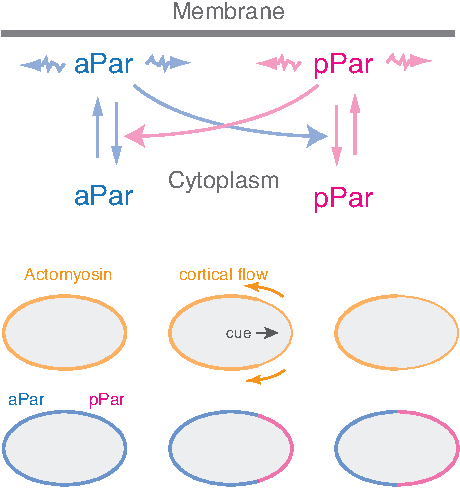
\includegraphics[width=\textwidth]{CElegansScheme-crop.pdf}
\end{column}
\end{columns}
\end{frame}


\begin{frame}{Movie: \emph{C.\ elegans} wild type}
\begin{center}
\hspace{-0.75 cm} NMY-2::GFP  \phantom{O thou}  mCherry::PAR-2 \phantom{O thouth} Merge
\movie[width=\textwidth,loop]{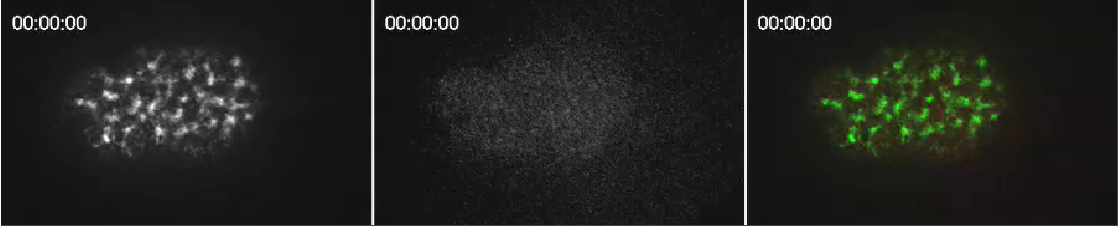
\includegraphics[width=\textwidth]{WildTypeStill-crop.pdf}}{PresentationFigsMovies/WildType.mp4}
\end{center}

\blfootnote{\tiny{Zonies et al. \emph{Development} (2010)}}
\end{frame}

\begin{frame}{Standard version of the story}
No flows in maintenance?

Gross paper
\end{frame}

\begin{frame}{Maintenance phase: a closer look}
\begin{columns}
\begin{column}{0.5\textwidth}
\movie[width=\textwidth,loop]{\includegraphics[width=\textwidth]{WildTypeFr1.jpg}}{PresentationFigsMovies/WildType.avi}
\pause
\includegraphics[width=\textwidth]{WTKymo_2.png}
\end{column}
\pause
\begin{column}{0.5\textwidth}
\includegraphics[width=0.9\textwidth]{LateMaintenanceK-crop.pdf}
\end{column}
\end{columns}
\end{frame}

\begin{frame}{Questions to answer}
Late maintenance: more myosin on anterior, steady A-directed flow
\begin{itemize}\pause
\item Is this a steady state? If so, how? \pause
\item Is this an \emph{attractive} steady state? Or does it depend on establishment? \pause
\item Can we understand this with a simple model?
\end{itemize}
\end{frame}

\begin{frame}{Questions to answer}
Late maintenance: more myosin on anterior, steady A-directed flow
\begin{itemize}
\item Is this a steady state?
\item \lightgray{Is this an \emph{attractive} steady state? Or does it depend on establishment?}
\item \lightgray{ Can we understand this with a simple model?}
\end{itemize}
\end{frame}

\begin{frame}{Late maintenance is (roughly) a steady state}
Use CDK-1 (RNAi) to expand maintenance phase; boundary actually moves towards posterior

\begin{center}
NMY-2::GFP

\movie[width=0.7\textwidth,loop]{\includegraphics[width=0.7\textwidth]{CDK1.jpg}}{PresentationFigsMovies/cdk-1RNAi_NMY2gfp.avi}
\end{center}

\end{frame}

\begin{frame}{Myosin boundary stable }
\begin{columns}
\begin{column}{0.4\textwidth}
\includegraphics[width=\textwidth]{MyosinBDCDK.pdf}
\end{column}
\begin{column}{0.6\textwidth}
\begin{center}
\phantom{123} Myosin -- last 4 minutes
\includegraphics[width=\textwidth]{CDK1MyosinLast4Mins.pdf}
\end{center}
\end{column}
\end{columns}
\vspace{0.5 cm}

Slight shift towards posterior; but still have A/P asymmetry
\end{frame}

\begin{frame}{Steady flow profile in CDK-1 embryos}
\begin{columns}
\begin{column}{0.3\textwidth}
\includegraphics[width=\textwidth]{CDK1Kymo.png}
\end{column}
\begin{column}{0.7\textwidth}
\begin{center}
\phantom{1234} Flows -- last 4 minutes
\includegraphics[width=0.9\textwidth]{CDK1FlowsLast4Mins.pdf}
\end{center}
\end{column}
\end{columns}
\vspace{0.5 cm}

Still see contraction into medial domain (nonzero flows)
\end{frame}

\begin{frame}{Questions to answer}
Late maintenance: more myosin on anterior, steady A-directed flow
\begin{itemize}
\item \lightgray{Is this a steady state? \checkmark}
\item Is this an \emph{attractive} steady state? Or does it depend on establishment?
\item \lightgray{ Can we understand this with a simple model?}
\end{itemize}
\end{frame}


\begin{frame}{Distinction between establishment and maintenance}
\begin{columns}
\begin{column}{0.5\textwidth}
Establishment phase
\begin{center}
\includegraphics[width=\textwidth]{EstablishmentBC.pdf}
\end{center}
\begin{itemize}
\item Pulsatile contractility (Michaux et al., 2018)
\item Governed by rho
\end{itemize}
\begin{center}
\includegraphics[width=0.8\textwidth]{EstablishmentMyosin.jpg}
\end{center}
\end{column}
\pause
\begin{column}{0.5\textwidth}
Maintenance phase
\includegraphics[width=\textwidth]{MaintenanceBC.pdf}
\begin{itemize}
\item Diffuse myosin clusters
\item Governed by CDC-42 (through MRCK)
\end{itemize}
\begin{center}
\includegraphics[width=0.8\textwidth]{MaintenanceMyosin.jpg}
\end{center}
\end{column}
\end{columns}
\end{frame}


\begin{frame}{Starting polarity from maintenance}
Disturb establishment by knocking down rho
\begin{itemize}
\item ECT-2 ts mutant $\rightarrow$ no cortical flows
\item Both cases: local zone of PAR-2 enrichment remains
\end{itemize}

\pause
\begin{center}
\hspace{-0.75 cm} NMY-2::GFP  \phantom{O thou}  mCherry::PAR-2 \phantom{O thouth} Merge
\movie[width=\textwidth,loop]{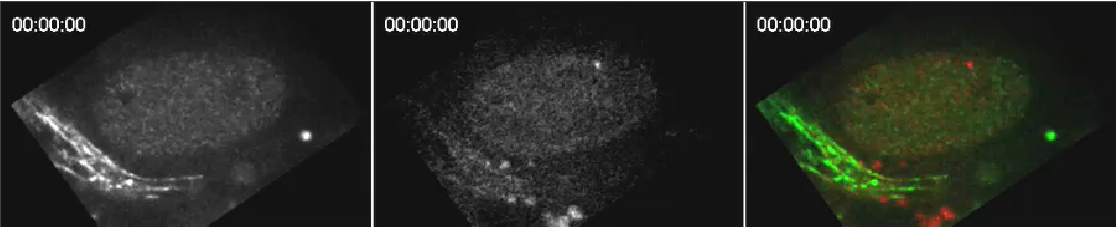
\includegraphics[width=\textwidth]{ZoniesFrame1.pdf}}{PresentationFigsMovies/ZoniesNMYEct2.mov}
\end{center}

Results in exactly the same boundary position!
\begin{itemize}
\item Requires CDC-42, MRCK
\pause 
\item Experiments by Charlie show maintenance is an error correction mechanism
\end{itemize}

\blfootnote{\tiny{Zonies et al. \emph{Development} (2010)}}
\end{frame}

\begin{frame}{Questions to answer}
Late maintenance: more myosin on anterior, steady A-directed flow
\begin{itemize}
\item \lightgray{Is this a steady state? \checkmark}
\item \lightgray{Is this an \emph{attractive} steady state? Or does it depend on establishment? \checkmark}
\item Can we understand this with a simple model?
\begin{itemize}
\item Account for aPAR/pPAR maintenance without flows
\item How to explain rescue?
\end{itemize}
\end{itemize}
\end{frame}


\begin{frame}{Maintenance model}
\includegraphics[width=\textwidth]{MaintenanceModel.pdf}
\end{frame}


\begin{frame}{Maintenance model without flows}
\begin{columns}
\begin{column}{0.5\textwidth}
Starting from end establishment
\begin{center}
\movie[width=\textwidth,loop]{\includegraphics[width=\textwidth]{SteadyStateNoFlow-crop.pdf}}{PresentationFigsMovies/NoFlowMiddle.avi}
\end{center}
\end{column}
\begin{column}{0.5\textwidth}
Starting from small asymmetry
\begin{center}
\movie[width=\textwidth,loop]{\includegraphics[width=\textwidth]{SteadyStateNoFlow-crop.pdf}}{PresentationFigsMovies/NoFlowRescue.avi}
\end{center}
\end{column}
\end{columns}
\pause
\vspace{0.5 cm}
Slow reaction-diffusion mechanism can ``pin'' boundary, but not in realistic time
\begin{itemize}
\item Consistent with experiment (MRCK = flows)
\end{itemize}
\end{frame}

\begin{frame}{Maintenance model without flows: conclusions}
\begin{center}
\includegraphics[width=0.9\textwidth]{SimsNoFlow.pdf}
\end{center}
aPAR/pPAR circuit can maintain stable boundary, but cannot rescue it (in realistic time)
\begin{itemize}
\item Consistent with experiment (MRCK = flows)
\end{itemize}
\end{frame}

\begin{frame}{Adding flows to maintenance model}
\begin{columns}
\begin{column}{0.5\textwidth}
\begin{center}
\includegraphics[width=\textwidth]{MaintenanceModelFlows.pdf}
\end{center}
\end{column}
\begin{column}{0.5\textwidth}
\begin{center}
\movie[width=\textwidth,loop]{\includegraphics[width=\textwidth]{InitialRunMaintFlow.pdf}}{PresentationFigsMovies/FlowRescue.avi}
\end{center}
\end{column}
\end{columns}
\pause
\vspace{0.5 cm}
No way to stop the build up of myosin!
\begin{itemize}
\item Need some inhibitor of contractility on anterior
\end{itemize}
\end{frame}

\begin{frame}{Adding flows to maintenance model: kymographs}
\begin{center}
\includegraphics[width=\textwidth]{MaintenanceFlowKymos.pdf}
\end{center}
\vspace{0.5 cm}
No way to stop the build up of myosin!
\begin{itemize}
\item Need some inhibitor of contractility on anterior
\end{itemize}
\end{frame}





\begin{frame}{Questions to answer}
Late maintenance: more myosin on anterior, steady A-directed flow
\begin{itemize}
\item \lightgray{Is this a steady state? \checkmark}
\item \lightgray{Is this an \emph{attractive} steady state? Or does it depend on establishment? \checkmark}
\item \lightgray{Can we understand this with a simple model? \xmark}
\item Can experiments identify the missing piece?
\item \lightgray{Does a re-informed model make the correct predictions?}
\end{itemize}
\end{frame}


\begin{frame}{Depleting branched actin gives hypercontractile state}
Treat with nocodazole to remove MT forces pulling on cap
\begin{itemize}
\item Hypothesis: branched actin halts myosin constriction
\item \red{Update movies}
\end{itemize}

\begin{center}
Wild type

\movie[width=0.52\textwidth,loop]{\includegraphics[width=0.52\textwidth]{CDK1.png}}{PresentationFigsMovies/cdk-1RNAi_NMY2gfp.avi}


\emph{arx-2} (RNAi)

\movie[width=0.52\textwidth,loop]{\includegraphics[width=0.52\textwidth]{Arx2RNAi.png}}{PresentationFigsMovies/arxRNAi_NMY2gfp.avi}
\end{center}

\end{frame}

\begin{frame}{Depleting branched actin gives hypercontractile state}

\begin{center}
\includegraphics[width=\textwidth]{WTArxStats.pdf}
\end{center}

\end{frame}

\begin{frame}{Depleting branched actin gives hypercontractile state}
Treat with nocodazole to remove MT forces pulling on cap

\begin{center}
\includegraphics[width=\textwidth]{NocoArxStats.pdf}
\end{center}

\end{frame}

\begin{frame}{Does rescue work without branched actin?}
\begin{columns}
\begin{column}{0.5\textwidth}
\begin{center}
ect-2 ts
\movie[width=\textwidth,loop]{\includegraphics[width=\textwidth]{ect2_ts_Still.jpg}}{PresentationFigsMovies/ect2_ts_e6.avi}
\end{center}
\end{column}
\begin{column}{0.5\textwidth}
\begin{center}
\phantom{123} ect-2 ts + arx-2 (RNAi)
\movie[width=\textwidth,loop]{\includegraphics[width=\textwidth]{ect2ts_arx2_Still.jpg}}{PresentationFigsMovies/ect2ts_arx2_e4.avi}
\end{center}
\end{column}
\end{columns}

\end{frame}

\begin{frame}{Does rescue work without branched actin?}
\begin{center}
\includegraphics[width=\textwidth]{KymosRescueArx.pdf}
\end{center}

\end{frame}


\begin{frame}{Rescue dynamics: a closer look}

\end{frame}

\begin{frame}{Conclusions and future work}
Maintenance phase ``rescue'' $\approx$ same pathway as establishment
\begin{itemize}
\item PAR-3 intrinsically bistable
\item PAR-2 ``invades'' based on excess cytoplasmic
\item Myosin inhibition by PAR-2 $\rightarrow$ further expansion
\item Boundary pinned when run low on PAR-2
\end{itemize}
Flow and myosin profiles out of whack in WT vs.\ model
\begin{itemize}
\item Better match: \emph{arx-2} (RNAi) embryos 
\item Branched actin inhibits contractility
\item Incorporate into model; match WT?
\end{itemize} 
\end{frame}

\end{document}
